%% HKUST unofficial poster template
% By Ching Ting Leung, class of 2025 in BEng

% Forked from Gemini theme
% https://github.com/anishathalye/gemini

% Required Compiler: LuaLaTeX

\documentclass[final]{beamer}

% ====================
% Packages
% ====================

\usepackage[T1]{fontenc}
\usepackage{lmodern}
\usepackage[size=custom,width=81,height=145,scale=1.0]{beamerposter} % default
%\usepackage[orientation=portrait,size=a1,scale=1.0]{beamerposter} % custom
% scale: scaling factor of all font

\usetheme{gemini}
\usecolortheme{Tuebingen} % Customize in beamercolorthemeTuebingen.sty

\usepackage{graphicx}
\usepackage{booktabs}
\usepackage{tikz}
\usepackage{pgfplots}
\pgfplotsset{compat=1.14}
\usepackage{anyfontsize}

\usepackage{url}
\usepackage{multicol}
\usepackage{balance}

% ====================
% Lengths
% ====================

% If you have N columns, choose \sepwidth and \colwidth such that
% (N+1)*\sepwidth + N*\colwidth = \paperwidth
\newlength{\sepwidth}
\newlength{\colwidth}
\setlength{\sepwidth}{0.03\paperwidth}
\setlength{\colwidth}{0.48\paperwidth}

\newcommand{\separatorcolumn}{\begin{column}{\sepwidth}\end{column}}

\setbeamertemplate{caption}{\raggedright\insertcaption\par}

\addtobeamertemplate{block begin}{\vskip -\bigskipamount}{}
\addtobeamertemplate{block end}{}{\vskip -\bigskipamount}

% ====================
% Title
% ====================

\title{Current State of Language Technologies in Sorbian Languages}

\author{Daniel Sobe \inst{1} \and Ivan Kraljevski \inst{2}}

\institute[shortinst]{\inst{1} Załožba za serbski lud, Budyšin / Foundation for the Sorbian people, Bautzen, Germany \and \inst{2} Fraunhofer Institute for Ceramic Technologies and Systems IKTS, Dresden, Germany}

% ====================
% Footer (optional)
% ====================

\footercontent{
  \href{https://zalozba.de}{https://zalozba.de} \hfill
  LT4All 2025, Paris \hfill
  \href{mailto:d.zoba@zalozba.de}{d.zoba@zalozba.de}}
% (can be left out to remove footer)

% ====================
% Logo (optional)
% ====================

% use this to include logos on the left and/or right side of the header:
\logoright{
\includegraphics[height=7cm]{00_z_01_SfdsV_Logo2015_CMYK_border.jpg}}
\logoleft{
\includegraphics[height=7cm]{00_z_02_FHG_Logo.png}}

% ====================
% Body
% ====================

\begin{document}

\begin{frame}[t]
\begin{columns}[t]
%\separatorcolumn

\begin{column}{\colwidth}

  \begin{block}{Speech recognition (HSB)}
    
    \center{Live subtitles of church services}

    \begin{figure}
        \centering
        
\includegraphics[width=\colwidth]{01_z_01_citanje.png}
        \caption{\url{https://www.youtube.com/@chroscancyrkej/streams}}
        \label{fig:webcaptioner}
    \end{figure}

    \center{Project owner: Foundation for the Sorbian people\cite{zalozba}}
    
  \end{block}


  \begin{block}{Machine translation (HSB \& DSB)}

    % \center{Webinterface for translation between German, Upper Sorbian and Lower Sorbian}

    \begin{figure}
        \centering
        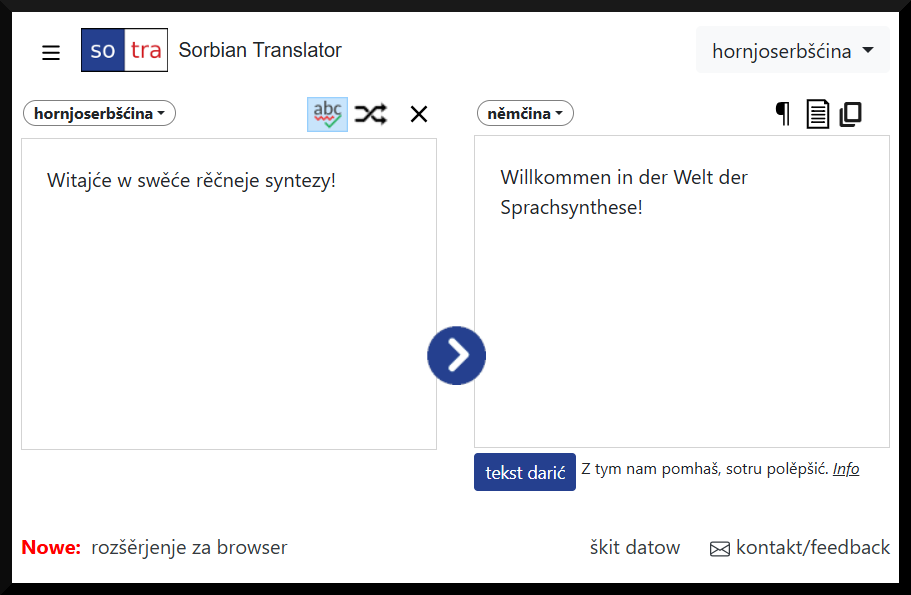
\includegraphics[width=0.7\colwidth]{02_z_01_sotra_rand.png}
        \caption{\url{https://sotra.app}}
        \label{fig:webcaptioner}
    \end{figure}

    \center{Project owner: Language Centre "Witaj" \cite{witaj}}

  \end{block}


  \begin{block}{Simultaneous translation (HSB)}

    \center{Combination of speech recognition and machine translation}

    \begin{figure}
        \centering
        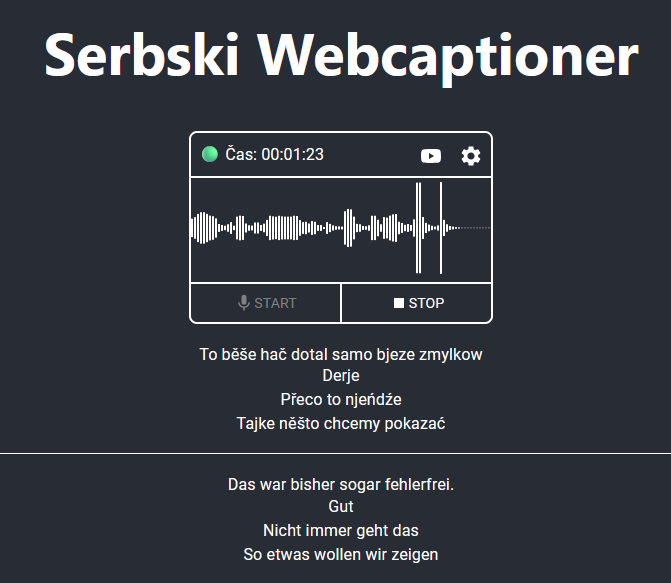
\includegraphics[width=0.7\colwidth]{03_z_01_webcaptioner_klein.png}
        \caption{Source code: \url{https://github.com/ZalozbaDev/webcaptioner-ng}}
        \label{fig:webcaptioner}
    \end{figure}

  \end{block}


  \begin{block}{Language research (HSB \& DSB)}  

    % \center{Research portals}

    \begin{figure}
        \centering
        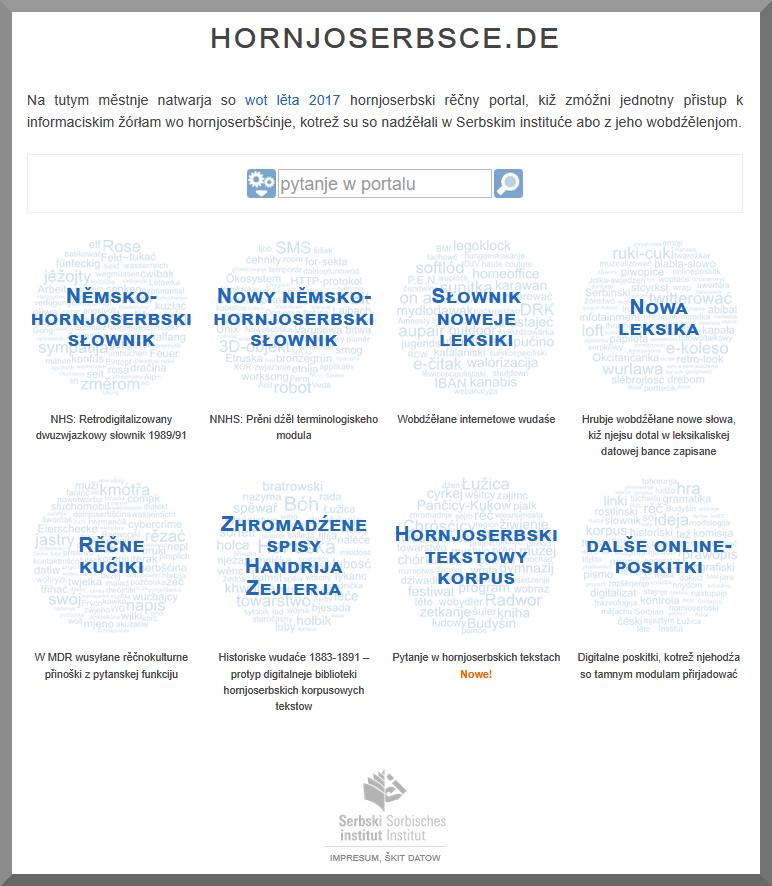
\includegraphics[width=0.7\colwidth]{04_z_01_hornjoserbsce_gross_rand.png}
        \caption{\url{https://hornjoserbsce.de/} and \url{https://dolnoserbski.de/}}
        \label{fig:hornjoserbsce}
    \end{figure}

    \center{Project owner: Sorbian institute \cite{institut}}

  \end{block}


\end{column}

%\separatorcolumn

\begin{column}{\colwidth}

  \begin{block}{Language practice (HSB)}

    %\center{Online dictionary}

    \begin{figure}
        \centering
        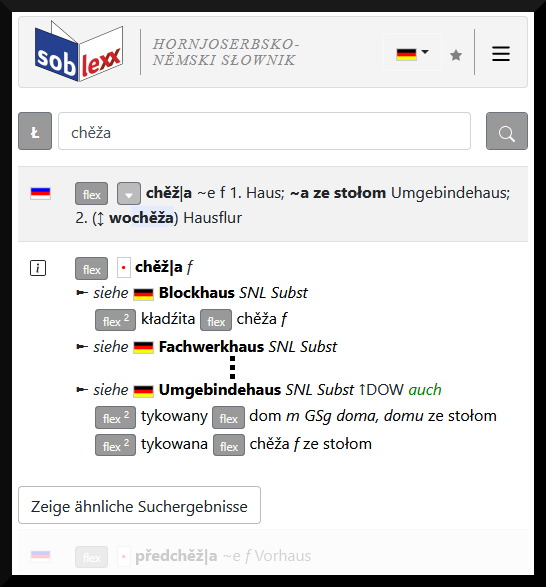
\includegraphics[width=0.7\colwidth]{05_z_01_soblex_suche_trunc_rand.png}
        \caption{(output truncated)}
        \label{fig:soblexsearch}
    \end{figure}

    %\center{Grammar tables}

    \begin{figure}
        \centering
        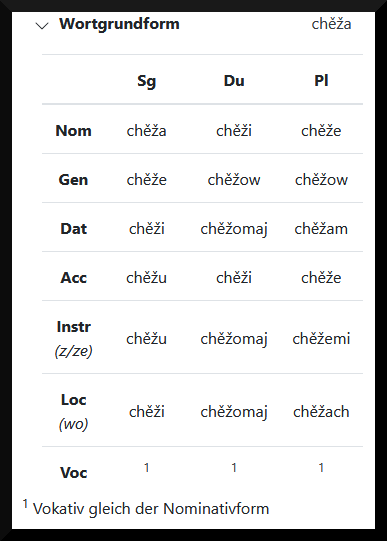
\includegraphics[width=0.5\colwidth]{05_z_02_soblex_klein_trunc_rand.png}
        \caption{\url{https://soblexx.de}}
        \label{fig:soblex}
    \end{figure}

    \center{Project owner: Bernhard Baier\cite{soblex}}
    
  \end{block}


  \begin{block}{Speech synthesis (HSB \& DSB)}

    \center{\textbf{MaryTTS (HSB and DSB) by the \textit{Sorbian institute} \cite{institut}}}

    \begin{figure}
        \centering
        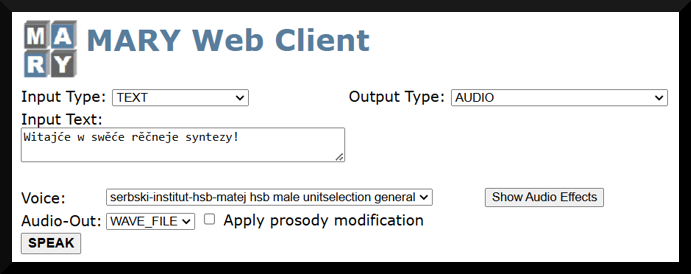
\includegraphics[width=0.7\colwidth]{06_z_01_marytts_small_rand.png}
        \caption{\url{https://tts-juro-matej.serbski-institut.de/}}
        \label{fig:marytts}
    \end{figure}

    % \center{Project owner: Sorbian institute\cite{institut}}    

    \center{\textbf{Coqui TTS (HSB) by \textit{Korla Baier\cite{bamborak}}}}

    \begin{figure}
        \centering
        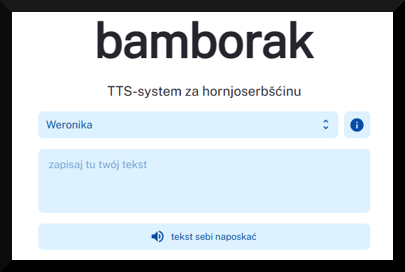
\includegraphics[width=0.5\colwidth]{06_z_02_bamborak_small_rand.png}
        \caption{\url{https://gaussia.de/bamborak/}}
        \label{fig:bamborak}
    \end{figure}
    
    % \center{Project owner: Korla Baier\cite{bamborak}}    

  \end{block}


%   \begin{block}{References}


%  \nocite{*}
   
    \begin{multicols}{2}
    %\balance
    % \vspace{1ex}    
    %\begin{center}
        \normalsize{\bibliographystyle{unsrt}\bibliography{07_z_01_poster}}
    %\end{center}

    \end{multicols}

  \end{block}
  
 \begin{block}{References}

\vspace{-5mm}
    \begin{multicols}{2} % Start two-column layout
        % \raggedbottom % Prevent automatic balancing of columns
        \begin{thebibliography}{99} 
            \bibitem{zalozba}
            Załožba za serbski lud\\
            \url{https://zalozba.de}\\
            \vspace{1mm}
            %\begin{center}
                {\qrcode[height=1in]{https://zalozba.de}}
           % \end{center}
            \vspace{1mm}
            
            \bibitem{witaj}
            Rěčny centrum Witaj\\
            \url{https://www.witaj-sprachzentrum.de/}\\
            \vspace{1mm}
            %\begin{flushleft}
                \qrcode[height=1in]{https://www.witaj-sprachzentrum.de/}
            %\end{flushleft}
            \vspace{45mm}

            % \columnbreak
            
            \bibitem{institut}
            Serbski institut\\
            % \vspace{40mm}
            \url{https://www.serbski-institut.de/}\\
            \vspace{1mm}
            %\begin{center}
                \qrcode[height=1in]{https://www.serbski-institut.de/}
            %\end{center}
            \vspace{1mm}
            
            \bibitem{soblex}
            Bernhard Baier\\
            \url{https://soblexx.de}\\
            \vspace{1mm}
            %\begin{center}
                \qrcode[height=1in]{https://soblexx.de}
            %\end{center}
            \vspace{1mm}
            
            \bibitem{bamborak}
            Korla Baier\\
            \url{https://gaussia.de/bamborak}\\
            \vspace{1mm}
            %\begin{center}
                \qrcode[height=1in]{https://gaussia.de/bamborak}
            %\end{center}
            \vspace{1mm}
            
            % Add more references as needed
        \end{thebibliography}
    \end{multicols}
\end{block}    





\end{column}

%\separatorcolumn
\end{columns}
\end{frame}

\end{document}
